\documentclass{standalone} % DO NOT CHANGE THIS
\usepackage{tikz}
\usepackage[utf8]{inputenc}
\usepackage{graphicx}
\usepackage{times}
\usepackage{amssymb}
\usetikzlibrary[arrows.meta, positioning,math, calc]

\begin{document}

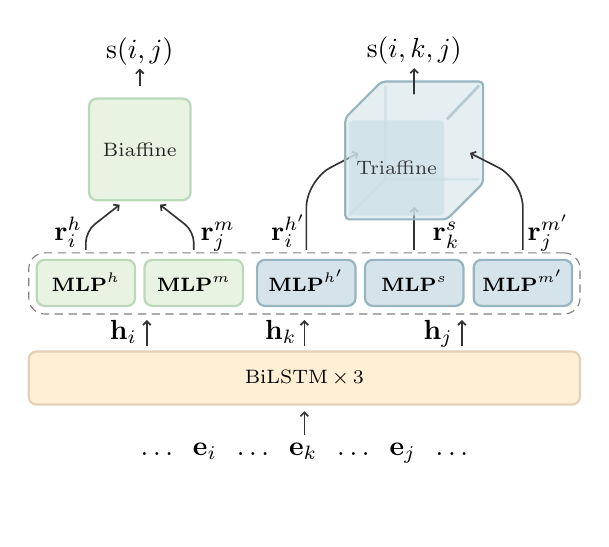
\begin{tikzpicture}[
    connect/.style={
            rounded corners=4pt,
            semithick,
            draw=black!80
        },
    arrow/.style={
            % >=latex,
            arrows = {-Straight Barb[length=0.5mm]},
            shorten >= 2pt,
            shorten <= 1.5pt,
            thin
        },
    inner arrow/.style={
            arrows = {-Straight Barb[length=0.4mm]},
            shorten >= 2pt,
            shorten <= 2pt,
            thin,
            draw=black!50
        },
    input/.style={
            rectangle,
            rounded corners=1mm,
            %   thick,
            thin,
            dashed,
            draw=none,
            % fill=white,
            minimum width=3.5cm,
            minimum height=0.6cm,
            %   fill=orange!10,
            %   draw=orange!40
            %   fill={rgb,255:red,255; green,239; blue,213},
            %   draw={rgb,255:red,225; green,209; blue,183},
        },
    share/.style={
            minimum height=0.5cm,
            %   fill=orange!10,
            %   draw=orange!40,
            fill={rgb,255:red,255; green,239; blue,213},
            %   fill,
            %   right color={rgb,255:red,204; green,223; blue,230},
            %   left color={rgb,255:red,228; green,242; blue,220},
            draw={rgb,255:red,225; green,209; blue,183},
            rounded corners=2mm,
        },
    task2/.style={
            minimum height=0.5cm,
            fill={rgb,255:red,228; green,242; blue,220},
            draw={rgb,255:red,187; green,217; blue,186},
            rounded corners=2mm,
        },
    label/.style={
            inner sep=0.5mm,
            fill=white,
            minimum height=0.5cm,
        },
    task1/.style={
            minimum height=0.5cm,
            fill={rgb,255:red,204; green,223; blue,230},
            draw={rgb,255:red,151; green,181; blue,191},
            rounded corners=2mm
        },
    inner lstm/.style={
            fill=white,
            rectangle,
            rounded corners=1mm,
            semithick,
            draw=black!50,
            fill opacity=0.8
        },
    cell/.style={
            inner sep=2mm,
            rectangle,
            rounded corners=1mm,
            semithick,
            draw=black!50,
        },
    ocell/.style={
            solid,
            minimum height=0.5cm,
            rectangle,
            rounded corners=1mm,
            thick
        },
    dep arrow/.style={
    arrows = {-Latex[round,open,length=8pt,width=6pt]},
    shorten >= 2pt,
    shorten <= 1.5pt,
    thick
    }
    ]
    \centering
    \node [input, inner sep=1pt] [minimum width=4.8cm] (input) at (0, 0) {$\ldots\;\; \mathbf{e}_i \;\;\ldots\;\; \mathbf{e}_k \;\;\ldots\;\; \mathbf{e}_j \;\;\ldots$};
    \node [inner sep=0mm] at ($(input.south) + (0, -0.5cm)$) {\textbf{}};
    % Concat
    \node [inner sep=0] (EmbedCat) at ($(input.north)$) {};

    %\scriptsize BiLSTM
    \node [share, ocell] [minimum width=7cm, minimum height=0.675cm, anchor=south] (lstm) at ($(input.north) + (0, 0.3cm)$) {\scriptsize BiLSTM$\, \times \, 3$};

    % \node [inner lstm][minimum width=6.8cm, minimum height=0.675cm, anchor=south] (inner lstm0) at ($(lstm.south) + (0, 0.1cm)$) {\scriptsize BiLSTM$\, \times \, 3$};

    \draw [arrow, connect] ($(EmbedCat.north) + (0cm, -0.15cm)$) -- ($(lstm.south) + (0cm, 0)$);

    \foreach \x in {0, ..., 2}{
            \tikzmath{
                integer \nx;
                \nx = \x + 1;
            }
        };
    % fisrt two mlps
    \node [share, fill=none, draw=gray, densely dashed] [minimum width=7cm, minimum height=0.775cm, anchor=south] (share-mlp) at ($(lstm.north) + (0cm, 0.455cm)$) {};
    \node [task2, ocell] [minimum width=1.25cm, minimum height=0.585cm, anchor=south west, fill opacity=0.85] (mlp-1-1-f) at ($(lstm.north west) + (0.1cm, 0.55cm)$) {};
    \node [task2, ocell] [minimum width=1.25cm, minimum height=0.585cm, anchor=south west, fill opacity=0.85] (mlp-1-1-b) at ($(lstm.north west) + (1.47cm, 0.55cm)$) {};
    \node [anchor=base] at  ($(mlp-1-1-f.south) + (0, 0.2cm)$)  {\scriptsize $\mathbf{MLP}^{h}$};
    \node [anchor=base] at  ($(mlp-1-1-b.south) + (0, 0.2cm)$)  {\scriptsize $\mathbf{MLP}^{m}$};

    % \draw [arrow, connect, rounded corners=1.2pt, shorten >= 2pt] ($(lstm.north -| mlp-1-1-b)$) -- ($(mlp-1-1-b.south)$);

    % \draw [arrow, connect, rounded corners=1.2pt, shorten >= 2pt] ($(lstm.north -| mlp-1-1-f)$) -- ($(mlp-1-1-f.south)$);

    \node [task2, ocell, fill=none, draw=none] [minimum width=1.75cm, minimum height=0.40cm, anchor=south east, fill opacity=0.5, draw opacity=0.6] (mlp-1-2-b) at ($(mlp-1-1-b.north east) + (0, 0.5cm)$) {};

    \node [task2, ocell, anchor=south, fill opacity=0.85, minimum height=1.29cm, minimum width=1.29cm, align=center] (mlp-1-2-f) at ($(mlp-1-1-f.north)!0.5!(mlp-1-1-b.north) + (0, 0.73cm)$) {\scriptsize Biaffine};

    \draw [arrow, connect] ($(mlp-1-1-b.north) + (0, 0.06cm)$) -- ($(mlp-1-1-b.north) + (0, 0.35cm)$) -- ($(mlp-1-2-f.south) + (0.2, 0)$);
    \draw [arrow, connect] ($(mlp-1-1-f.north) + (0, 0.06cm)$) -- ($(mlp-1-1-f.north) + (0, 0.35cm)$) -- ($(mlp-1-2-f.south) + (-0.2, 0)$);

    % second two mlps
    \node [task1, ocell] [minimum width=1.25cm, minimum height=0.585cm, anchor=south east, fill opacity=0.85] (mlp-2-1-f) at ($(lstm.north east) + (-2.85cm, 0.55cm)$) {};
    \node [task1, ocell] [minimum width=1.25cm, minimum height=0.585cm, anchor=south east, fill opacity=0.85] (mlp-2-1-b) at ($(lstm.north east) + (-1.48cm, 0.55cm)$) {};
    \node [task1, ocell] [minimum width=1.25cm, minimum height=0.585cm, anchor=south east, fill opacity=0.85] (mlp-2-1-bb) at ($(lstm.north east) + (-0.1cm, 0.55cm)$) {};
    \node [anchor=base] at  ($(mlp-2-1-f.south) + (0, 0.2cm)$)  {\scriptsize $\mathbf{MLP}^{h'}$};
    \node [anchor=base] at  ($(mlp-2-1-b.south) + (0, 0.2cm)$)  {\scriptsize $\mathbf{MLP}^{s}$};
    \node [anchor=base] at  ($(mlp-2-1-bb.south) + (0, 0.2cm)$)  {\scriptsize $\mathbf{MLP}^{m'}$};

    \draw [arrow, connect, rounded corners=10pt] ($(mlp-2-1-f.north) + (0, 0.06cm)$) -- ($(mlp-2-1-f.north) + (0, 1cm)$) -- ($(mlp-2-1-b.north) + (-0.875, 0.5) + (0.23, 0.23) + (0, 0.645)$);
    \draw [arrow, connect] ($(mlp-2-1-b.north) + (0, 0.06cm)$) -- ($(mlp-2-1-b.north) + (0, 0.5cm) + (0, 0.23)$);

    \begin{scope}[]
        \begin{scope}[transparency group, opacity=0.3, densely dashed]
            \draw [task1, fill=none, rounded corners=0.1mm] ($(mlp-2-1-b.north) + (-0.825, 0.55)$) -- ($(mlp-2-1-b.north) + (-0.365, 1.01)$) -- ($(mlp-2-1-b.north) + (0.825, 1.01)$);

            \draw [task1, fill=none, rounded corners=0.1mm] ($(mlp-2-1-b.north) + (-0.365, 2.20)$) -- ($(mlp-2-1-b.north) + (-0.365, 1.01)$);
        \end{scope}
    \end{scope}

    \filldraw[task1, ocell, fill opacity=0.5, rounded corners=0.5mm] ($(mlp-2-1-b.north) + (-0.875, 0.5)$) -- ($(mlp-2-1-b.north) + (0.415, 0.5)$) -- ($(mlp-2-1-b.north) + (0.875, 0.96)$) -- ($(mlp-2-1-b.north) + (0.875, 2.25)$) -- ($(mlp-2-1-b.north) + (-0.415, 2.25)$) -- ($(mlp-2-1-b.north) + (-0.875, 1.79)$) -- cycle;

    \node [anchor=south west, minimum height=1.29cm, minimum width=1.29cm, draw=none] (triaffine) at ($(mlp-2-1-b.north) + (-0.875, 0.5)$) {};

    \node [fill={rgb,255:red,204; green,223; blue,230}, fill opacity=0.75, minimum height=1.21cm, minimum width=1.21cm, draw=none, rounded corners=0.5mm, align=center, inner sep=0.1mm] at ($(triaffine) + (0, 0)$) {\scriptsize Triaffine};

    \begin{scope}[]
        \begin{scope}[transparency group, opacity=0.6]
            \draw [task1, fill=none, rounded corners=0.1mm] ($(mlp-2-1-b.north) + (0.825, 2.2)$) -- ($(mlp-2-1-b.north) + (0.415, 1.77)$);
            % \draw [task1, fill=none, rounded corners=0.1mm] ($(mlp-2-1-b.north) + (0.825, 2.2)$) -- ($(mlp-2-1-b.north) + (0.415, 1.77)$) -- ($(mlp-2-1-b.north) + (-0.825, 1.77)$);
            % \draw [task1, fill=none, rounded corners=0.1mm] ($(mlp-2-1-b.north) + (0.415, 1.77)$) -- ($(mlp-2-1-b.north) + (0.415, 0.55)$);
        \end{scope}
    \end{scope}

    \draw [arrow, connect, rounded corners=10pt] ($(mlp-2-1-bb.north) + (0, 0.06cm)$) -- ($(mlp-2-1-bb.north) + (0, 1cm)$) -- ($(mlp-2-1-b.north) + (0.415, 0.5) + (0.23, 0.23) + (0, 0.645)$);
    % \fill[fill opacity=0.5, fill=white] ($(mlp-2-1-b.north) + (0.415, 0.5) + (0.23, 0.23) + (0, 0.645)$) ellipse [x radius=0.014cm, y radius=0.05cm];

    %  LSMT -> MLP
    \draw [arrow, connect, rounded corners=1.2pt, shorten >= 2pt] ($(lstm.north) + (0cm, 0)$) -- ($(share-mlp.south) + (0cm, 0)$);
    \draw [arrow, connect, rounded corners=1.2pt, shorten >= 2pt] ($(lstm.north) + (-2cm, 0)$) -- ($(share-mlp.south) + (-2cm, 0)$);
    \draw [arrow, connect, rounded corners=1.2pt, shorten >= 2pt] ($(lstm.north) + (2cm, 0)$) -- ($(share-mlp.south) + (2cm, 0)$);
    \node[anchor=base] at ($(share-mlp.south) + (-2.3cm,-0.32cm) $) (label-h1) {$\mathbf{h}_{i}$};
    \node[anchor=base] at ($(share-mlp.south) + (-0.3cm,-0.32cm) $) (label-h2) {$\mathbf{h}_{k}$};
    \node[anchor=base] at ($(share-mlp.south) + (1.7cm,-0.32cm) $) (label-h53) {$\mathbf{h}_{j}$};

    % label
    % \node at ($(input.west) + (-2.18cm,0) $) (label-input) {$\mathbf{Input}$};
    % \node at ($(lstm.west) + (-0.85cm,0) $) (label-encoder) {$\mathbf{Encoder}$};
    % \node at ($(mlp-1-1-f.west) + (-1.22cm,0) $) (label-mlp-left) {$\mathbf{MLP}$};

    \node[anchor=base] at ($(share-mlp.north) + (-3cm,0.15cm) $) (label-r1) {$\mathbf{r}_{i}^{h}$};
    \node[anchor=base] at ($(share-mlp.north) + (-1.1cm,0.15cm) $) (label-r2) {$\mathbf{r}_{j}^{m}$};
    \node[anchor=base] at ($(share-mlp.north) + (-0.2cm,0.15cm) $) (label-r3) {$\mathbf{r}_{i}^{h'}$};
    \node[anchor=base] at ($(share-mlp.north) + (1.8cm,0.15cm) $) (label-r4) {$\mathbf{r}_{k}^{s}$};
    \node[anchor=base] at ($(share-mlp.north) + (3.1cm,0.15cm) $) (label-r5) {$\mathbf{r}_{j}^{m'}$};


    \node[anchor=base] at ($(mlp-1-2-f.north) + (0cm,0.5cm) $) (label-biaffine) {$\mathrm{s}(i,j)$};
    \node[anchor=base] at ($(triaffine.north -| mlp-2-1-b) + (0,0.75cm) $) (label-triaffine) {$\mathrm{s}(i,k,j)$};

    % \fill[fill opacity=0.5, fill=white] ($(triaffine.north -| mlp-2-1-b) + (0, 0.26cm)$) ellipse [x radius=0.05cm, y radius=0.014cm];

    \draw [arrow, connect, rounded corners=1.2pt, shorten >= 2pt] ($(label-biaffine.south) + (0, -0.2cm) $) -- ($(label-biaffine.south) + (0, 0.15cm) $);
    \draw [arrow, connect, rounded corners=1.2pt, shorten >= 2pt, line cap=round] ($(label-triaffine.south) + (0, -0.3cm) $) -- ($(label-triaffine.south) + (0, 0.15cm) $);

    % input arc
    % \draw [arrow] [out=-30,in=-150] ($(input.south west) + (1.05cm, 0.15cm)$) to ($(input.south east) + (-1.15cm, 0.15cm)$);
    % \draw [arrow] [out=-30,in=-150] ($(input.south west) + (1.05cm, 0.15cm)$) to ($(input.south east) + (-2.35cm, 0.15cm)$);
\end{tikzpicture}
\end{document}